\section{方法概览}
\label{section:overview}

为应对流水线阶段不均衡和训练数据动态性带来的挑战，
我们提出动态交错流水线（\underline{D}ynamic \underline{I}nterleaved \underline{P}ipeline，\sys{}），一个旨在优化 LMM 流水线并行的动态模态感知调度框架。
\sys{} 建立在三项关键设计原则之上：
通过异步生成调度来隐藏搜索延迟，
通过模态感知划分从源头缓解不均衡，
并通过分解式搜索算法高效找到高质量流水线调度。

\subsection{设计原则}
\label{section:design-decisions}

\begin{figure}[b]
    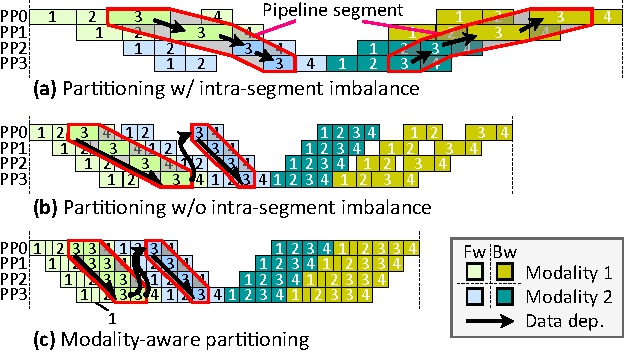
\includegraphics[width=1.0\columnwidth]{./figures/svg/schedule_observations.pdf}
    \caption{
        \S\ref{section:design-decisions}中各划分方案的示意图。
        方框中的数字表示微批次。
        \textbf{(a)} 非模态感知划分将不同模态的阶段放在同一个流水线段中，造成段内不均衡。
        \textbf{(b)} 分离式划分为每种模态分配独立流水线段，消除段内不均衡。
        \textbf{(c)} 模态感知数据分批进一步将微批次拆分为更小、特定于模态的子微批次，从而平衡不同流水线段之间的工作负载。
    }
    \label{figure:schedule-observations}
\end{figure}

\heading{异步调度生成}
与依赖静态或预计算调度的传统方法不同，为了处理 LMM 数据的动态特性，\sys{} 采用在线异步策略。
对于每个即将处理的数据批次，它并发、即时地生成定制流水线调度，从而有效适应多模态数据不断波动的计算需求。
这一过程包括数据预取和调度搜索，并在空闲 CPU 资源上异步运行，与 GPU 上的主要训练工作进程并行。由于不处于关键路径上，我们的方法可在不引入显著开销的情况下获得处理动态数据所需的适应能力。

\heading{模态感知划分}
如\S\ref{section:dynamic-imbalance}所述，LMM 训练效率低下的主要根源是不同模态模块之间动态变化的计算不均衡。
这种动态不均衡会造成不规则的阶段延迟，使流水线气泡难以消除。
为此，\sys{} 通过尽量缩小阶段延迟差异，从源头减少流水线气泡。
具体做法是将不同模态模块的计算划分到宽度相同的\emph{流水线段}中。
我们的方法由两项关键技术指导：

\textbf{\ding{172} 通过分离式划分消除段内不均衡。}
一个\emph{流水线段}是一组分布在全部 $P$ 个流水线秩上的连续阶段。
例如，\figref{figure:schedule-observations}a 中编号为“3”的四个前向阶段构成一个流水线段，
其对应的反向阶段则构成另一个流水线段。
我们观察到，将不同模态模块的阶段放在同一流水线段中（\figref{figure:schedule-observations}a）本质上是低效的。由于视觉阶段和语言阶段的计算成本不同，而且对数据比例（例如图像数与 token 数）的敏感程度也不同，将它们混合会在流水线秩之间造成不可避免的延迟差异。我们的第一项原则是强制采用\emph{分离式划分}（\figref{figure:schedule-observations}b），使每个模态模块占用各自专用的流水线段。这消除了流水线气泡的一个主要来源。对于 ViT 2B + LM 5B 模型（\S\ref{section:dynamic-imbalance}），仅这一策略相较最佳混合划分方案就能将性能提高 13.1\%。

\textbf{\ding{173} 通过模态感知分批消除段间不均衡。}
分离模态之后，还必须平衡各模态流水线段之间的工作负载。我们的第二项原则是将微批次内的数据划分为更小、特定于模态的\emph{子微批次}（\figref{figure:schedule-observations}c）。例如，如果整个视觉编码器阶段慢于某个 LM 阶段，就可以用更小的子微批次处理图像。
这样一来，编码器可以执行多个更短的阶段，并可调整每个编码器阶段的延迟，使其更好地匹配单个 LM 阶段的延迟。
这种模态感知分批方法可缩小整条流水线上的延迟差异，实现更为全局均衡且高效的调度。

\heading{分解式、可扩展的调度搜索}
调度搜索问题可以表述为一个整体式整数线性规划（ILP）问题，并使用现成求解器求解~\cite{highs,gurobi}。
这种方法精确，却难以用于实时场景，求解通常需要数分钟甚至数小时~\cite{recycle-sosp24}。
为满足一次训练迭代的严格时间预算（通常为 10--60 秒，\figref{figure:e2e-perf}b），我们采用分治策略，将复杂搜索问题分解为一系列更简单、更易处理的子问题。如\figref{figure:plan-searcher}所示，搜索器在一个三阶段循环中反复迭代，并在每一步应用专门设计的启发式方法：

\textbf{\ding{172} 流水线段重排（\S\ref{section:segment-reordering}）：}首先确定流水线段的最优处理顺序。我们使用蒙特卡洛树搜索（MCTS）高效探索庞大的排列空间，找出有潜力的流水线段顺序。

\textbf{\ding{173} 流水线阶段交错（\S\ref{section:stage-interleaving}）：}在流水线段顺序固定后，再排列相应的前向和反向流水线阶段。一个快速的双队列贪心算法对这些阶段进行交错，以尽量减少流水线气泡并紧密地填充调度。

\textbf{\ding{174} 逐层内存优化（\S\ref{section:memory-optimization}）：}最后，在调度结构固定后，分别优化每个流水线秩的内存使用。该阶段为所有模型层选择节省内存的策略（例如激活检查点与卸载），以尽量减小数据动态性引起的内存使用波动，并优化端到端迭代延迟。

整个循环可以在不同 CPU 线程之间高度并行，从而确保搜索过程能随可用 CPU 资源扩展，并服务于大型分布式训练集群。

\subsection{系统工作流}
\label{section:dip-overview}

上述原则由 \sys{} 训练规划器统一协调。该规划器由三个主要组件组成：模态感知划分器（\S\ref{section:modality-aware-partitioning}）、流水线调度搜索器（\S\ref{section:pipeline-schedule-searcher}）和训练仿真器（\S\ref{section:multimodal-training-simulator}）。

\begin{figure}[t]
    
\includegraphics[width=0.95\columnwidth]{./figures/svg/overview.pdf}
    \caption{
        \sys{} 的整体工作流。
        训练开始前，模型块划分器将 LMM 划分为模型块。
        每次训练迭代期间，\sys{} 异步执行一个四阶段在线规划过程。
    }
    \label{figure:overview}
\end{figure}

\begin{figure}[t]
    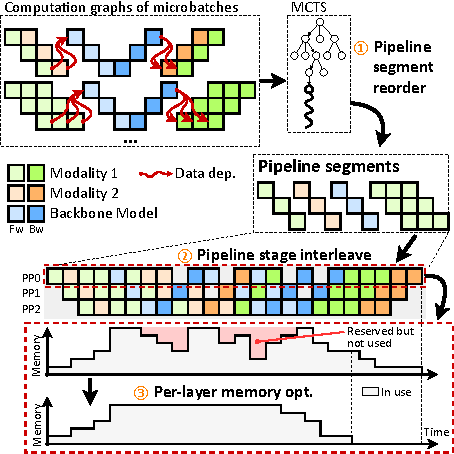
\includegraphics[width=1\columnwidth]{./figures/svg/plan_searcher.pdf}
    \caption{
        \sys{} 流水线调度搜索器的工作流。
    }
    \label{figure:plan-searcher}
\end{figure}

如\figref{figure:overview}所示，整体工作流分两个时期进行。
模态感知划分器包含一个离线模型块划分器和一个在线子微批次划分器。
\textbf{训练开始前，}模型块划分器根据我们的分离式划分原则将 LMM 划分为多个模型块，并把它们分布到指定 GPU 上。
\textbf{训练期间，}所有模型块都静态放置在各自的 GPU 工作进程上，底层网络拓扑（例如 NCCL 连接）也随之固定。
每次迭代中，规划器执行以下四阶段过程：

\textbf{\ding{172} 元数据预取：}规划器获取下一个批次的元数据（例如 token 数和图像数）。

\textbf{\ding{173} 自适应微批次划分：}子微批次划分器根据这些元数据，把微批次拆分为更小、特定于模态的子微批次，以实现段间负载均衡。

\textbf{\ding{174} 流水线调度搜索：}流水线调度搜索器以仿真器给出的性能估计为指导，运行三阶段算法，为生成的子微批次寻找最优调度。

\textbf{\ding{175} 运行时部署：}最佳调度被编译为执行计划，并下发到分布式训练运行时执行。
